\documentclass[10pt]{article}

\usepackage{float}
%\topmargin=0cm
\topmargin=-2cm
\addtolength{\textheight}{6.5cm}
\addtolength{\textwidth}{2.0cm}
\usepackage{graphicx}
\usepackage[T1]{fontenc}


\begin{document}

\section*{Student Information } 
Full Name : Yavuz Selim Yesilyurt \\
Id Number : 2259166 \\

\section*{Answer 1}
\hspace{4mm}	
Packet numbers of the packets used for 3-way handshake protocol that initiates the first TCP connection are 1, 2 and 3 respectively. 1st packet's segment number is 0 and its port numbers are 41248 in client side and 80 on server side. 2nd packet's segment number is 0 and its port numbers are 80 in client side and 41248 on server side. 3rd packet's segment number is 1 and its port numbers are 41248 in client side and 80 on server side.

\section*{Answer 2}
\hspace{4mm}	
HTTP GET request for "wireshark\_assignment2.png" was sent on 16th packet. After GET request, first 5 packet numbers and segment numbers of all TCP packets transferring the "wireshark\_assignment2.png" can easily be seen with the packet relating lines and figures according to conversations, on the "no." column of the trace file. According to these figures, the packet numbers of first 5 packets that carry image data are 21, 23, 25, 27 and 29. Corresponding ACK segments' packet numbers are 22, 24, 26, 28 and 34 respectively and corresponding data amount they acknowledged can be found with subtracting segment sequence number from ACK number on corressponding ACK segment. Making the computation:

\begin{center}
$7747 - 6373 = 1374$ for 1st ACK segment (22) \\
$9121 - 7747= 1374$ for 2nd ACK segment (24) \\
$10495 - 9121 = 1374$ for 3rd ACK segment (26) \\
$11869 - 10495 = 1374$ for 4th ACK segment (28) \\
$13243 - 11869 = 1374$ for 5th ACK segment (34) \\
\end{center}

Following table shows packet number, segment number, ACK packet number, and ACKed data columns: \\

\begin{table}[H]
\small
\centering
\begin{tabular}{|c|c|c|c|}	
\hline
Packet Number & Segment Number & ACK Packet Number & ACKed data column \\
\hline 
21 & 6373 & 22 & 1374 \\			
23 & 7747 & 24 & 1374 \\
25 & 9121 & 26 & 1374 \\
27 & 10495 & 28 & 1374 \\
29 & 11869 & 34 & 1374 \\
\hline 
\end{tabular}
\end{table}

\section*{Answer 3}
\hspace{4mm}	
First TCP data packet that is sent to the server is 21st packet with time $0.084727512$ and last acknowledgement packet that is received at the server side is 75th packet with time $0.173950634$, so it takes: 
\begin{center}
$0.173950634 - 0.084727512 = 0.08922312199999999$
\end{center}

Amount of time to transfer "wireshark\_assignment2.png" image data. Round Trip Time vs Time graph of related TCP packets is as follows:

\begin{figure}[H]
    \centering
    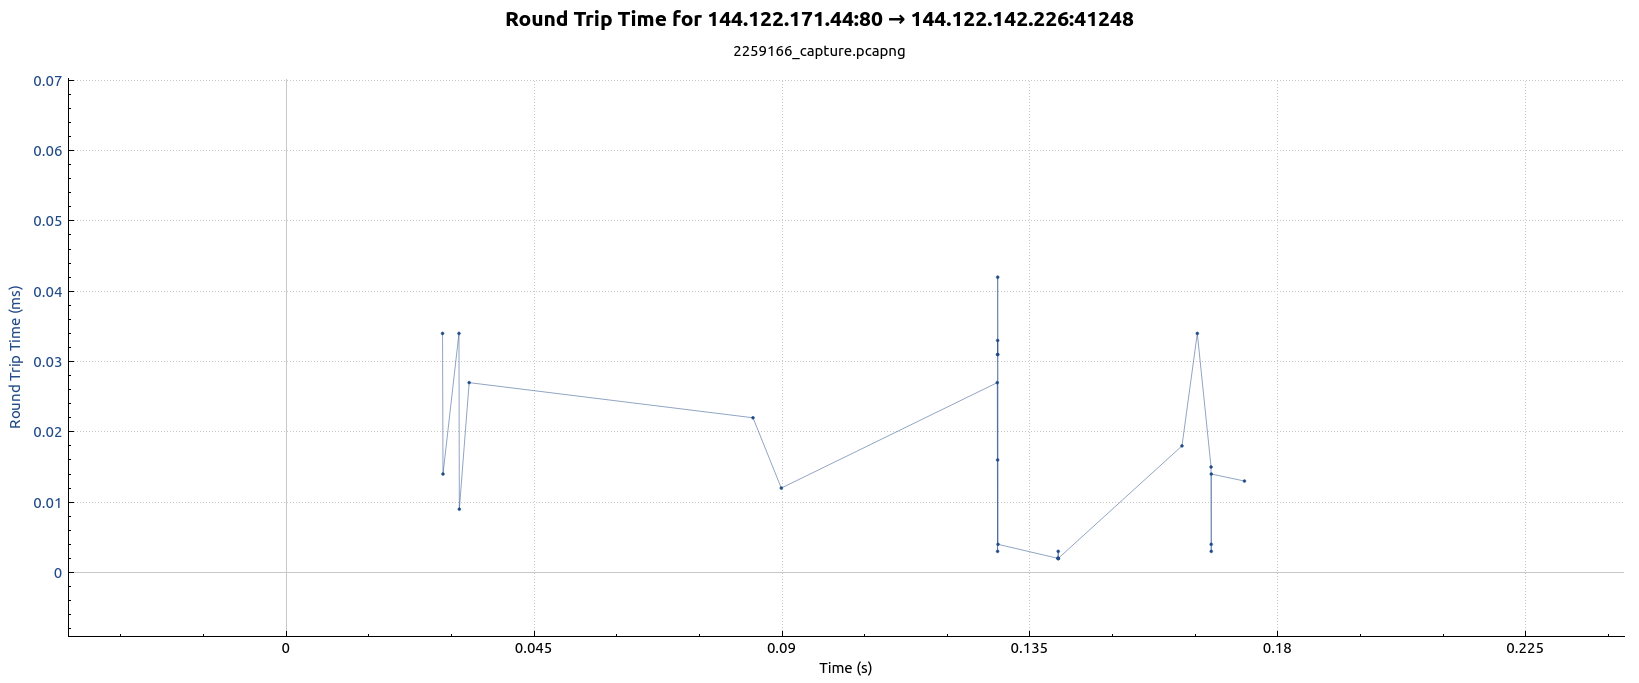
\includegraphics[scale=0.32]{graph.png}
    \caption{RTT vs Time}
\end{figure}



\section*{Answer 4}
\hspace{4mm}	
To be able to see if there is any kind retransmitted segments in output or not, one needs to check all kinds of TCP retransmissions so following filtering on trace file can be applied:
\begin{center}
"tcp.analysis.retransmission || tcp.analysis.fast\_retransmission || tcp.analysis.spurious\_retransmission"
\end{center}
After applying this filtering it can easily be seen that, yes, there is just one packet which is retransmitted. It is a TCP Spurious Retransmission packet with packet number = 56 and segment number = 2749.

\end{document}

​

